\documentclass[../main.tex]{subfiles}


\begin{document}
	\section{Práce se senzory}

	\subsection{Enkóder}
	Enkóder je senzor nezbytný k přesnému pohybu robota, jelikož měří otáčky jeho kol. Díky tomu jde (s dobrou přesností) určit, kde se robot nachází, a přizpůsobit tomu i naše programy.

	Jeden z nejčastějších typů enkóderů je optický enkóder. Funguje na principu světelného senzoru, na který svítí světlo (většinou lazer). Otáčením kolečka se senzor postupně zakrývá/odkrývá a touto změnou je tedy možné určit, že se kolečko otočilo.

	\begin{figure}[h!]%
		\centering%
		
\includegraphics[width=0.25\linewidth]{../Images/03/encoder-through.pdf}
		\hspace{.15\textwidth}%
		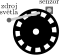
\includegraphics[width=0.25\linewidth]{../Images/03/encoder-blocked.pdf}
		\caption{Polohy optického enkóderu; nalevo světlo propouští, napravo blokuje.}
	\end{figure}

	\subsection{Světelný senzor}

	\subsection{Senzor nárazu}

\end{document}
